\documentclass[a4paper, 12pt]{article}

\usepackage{pgf}

% Used to reference the figures correctly at the top
% Also to center the captions on figures tables ->  justification=centering
\usepackage[hypcap=true]{caption}

\usepackage[numbers]{natbib}

% In order to load figures, images
\usepackage{graphicx}

% In order to inlcude [H] for figures
\usepackage{float}

% Used to draw the neural network
\usepackage{tikz}
\usetikzlibrary{chains, positioning, decorations.pathreplacing, arrows}
\def\layersep{3cm}

% Packages necessary for greek letters
\usepackage[utf8]{inputenc}
\usepackage[greek, english]{babel}  % Last language is the default
\usepackage[LGR, T1]{fontenc}

% Used to align equations
\usepackage{amsmath, amssymb}

% Used to make equations,figures appear with section number in front
\numberwithin{equation}{section}
\numberwithin{figure}{section}
\numberwithin{table}{section}

% Colors
\usepackage{xcolor}
\definecolor{darkred}{RGB}{200, 0 ,0}

% Used to ref click on TOC i could also use hidelinks to remove borders around reference
\usepackage{hyperref}
\hypersetup{colorlinks=true, linkcolor=blue, urlcolor=darkred, citecolor=}

% Add fields into the PDF
\hypersetup{
	pdfauthor=Tryfon Tsakiris,
	pdftitle=Deep Learning Frameworks' Effectiveness and Efficiency for Time Series Prediction, pdfsubject=Bachelor Thesis
}

% Used to add dots in sections at TOC
\usepackage{tocloft}
\renewcommand{\cftsecleader}{\cftdotfill{\cftdotsep}} 

% Include one more subsubsbusection
\usepackage{titlesec}
\titleformat{\paragraph}[hang]{\normalfont\normalsize\bfseries}{\theparagraph}{1em}{}
\titlespacing*{\paragraph}{0pt}{3.25ex plus 1ex minus .2ex}{1em}

% Increase numbering in TOC and etc
\setcounter{tocdepth}{4}
\setcounter{secnumdepth}{4}

% Used to generate plots 
\usepackage{pgfplots}
\pgfplotsset{width=10cm, compat=1.9}

% for my todo
\usepackage[colorinlistoftodos]{todonotes}
\newcommand{\mytodo}[2][]{\todo[#1, color=red!55]{#2}}

% booktabs: prettier tables, threeparttable: for caption aligment
%\usepackage{booktabs, caption, threeparttable}
\usepackage{booktabs}

% to set width of columns
\usepackage{array}
\newcolumntype{L}[1]{>{\raggedright\arraybackslash}m{#1}}

% used to stretch tables and make them have more space -- default is 1
\renewcommand{\arraystretch}{1.2}

% For abbrevations as 2columns
%\usepackage{enumitem}
%\newlist{abbrv}{itemize}{1}
%\setlist[abbrv,1]{label=,labelwidth=1in,align=parleft,itemsep=0.1\baselineskip,leftmargin=!}

% Pictures folder
\graphicspath{{figures/}}

\begin{document}
	
	% Remove numbering from title, abstract, acknowledgments
	\pagenumbering{gobble}
	
	% Custom title
	\begin{titlepage}
		
		\centering
		\includegraphics[scale=0.12, keepaspectratio]{uth.jpg}\\
		\vspace*{1cm}
		{\Large University of Thessaly}\\
		\vspace*{0.5cm}
		{\Large Department of Electrical and Computer Engineering}\\
		\vspace*{1cm}
		{\Large\bfseries{Deep Learning Frameworks' Effectiveness and Efficiency for Time Series Prediction\par}}
		% The below command adds two horizontal lines that are split by space
		\noindent\makebox[3cm]{\hrulefill} \hfill\makebox[3cm]{\hrulefill}\\
		\vspace*{0.5cm}
		{\large by\par}
		\vspace{0.3cm}
		{\large Tryfon Tsakiris\par}
		\vspace*{2cm}
		{\normalsize A thesis submitted for the partial fulfillment of the requirements for the bachelor degree in Electrical and Computer Engineering\par}
		\vspace*{2cm}
		{\large Supervised by\\[0.3cm] Dimitrios Katsaros, Assistant Professor\\ Lefteris Tsoukalas, Professor\par}
	\end{titlepage}
	
	% Start numbering again
	\pagenumbering{arabic}
	
	\section*{\textgreek{Περίληψη}}
	
	\begin{otherlanguage}{greek}
		Η αποτελεσματικότητα και ταχύτητα πρόβλεψης των τιμών μιας χρονοσειράς είναι σημαντική σε μια πληθώρα περιοχών όπως στα χρηματιστήρια, σεισμικές μελέτες και δίκτυα αισθητήρων. Ο στόχος της	παρούσας πτυχιακής εργασίας, είναι να αντιμετωπίσει αυτό το συγκεκριμένο πρόβλημα χρησιμοποιώντας τεχνικές βαθιάς μάθησης (\textlatin{deep learning)} και να διευρευνήσει την αποτελεσματικότητα (ακρίβειας) πρόβλεψης και την ταχύτητα	εκπαίδευσης και πρόβλεψης των κυριοτέρων βιβλιοθηκών βαθιάς μάθησης (\textlatin{deep learning)}. Εστιάζουμε στα \textlatin{\textit{ "Long Short-Term Memory" (LSTM)}} και \textlatin{\textit{"Gated Recurrent Unit" (GRU)}} νευρωνικά δίκτυα που είναι παράγωγα των \textlatin{\textit{"Recurrent  Neural Networks" (RNN)}} και είναι ειδικά σχεδιασμένα για να χειρίζονται ακολουθίες δεδομένων, όπως μια χρονοσειρά. Η υλοποίηση των μοντέλων πρόβλεψης έγινε με χρήση της υψηλού επιπέδου βιβλιοθήκης βαθιάς μάθησης \textit{\textlatin{Keras}},
		η οποία επιτρέπει την χρήση διαφορετικών πιο χαμηλού επιπέδου βιβλιοθηκών βαθιάς μάθησης (\textit{\textlatin{Tensorflow, Theano, CNTK}}) ως την υποστηρικτική μηχανή της, η οποία καθιστά εφικτή την δίκαιη σύγκριση μεταξύ τους.
	\end{otherlanguage}
	
	\newpage
	
	% Abstract and Acknowledgments
	\section*{Abstract}
	
	The speed and efficiency of predicting the values of a time series is important in a variety of areas such as stock exchanges, seismic studies and sensor networks. The aim of this dissertation is to tackle this specific task with deep learning and explore the prediction efficiency and the speed of training and prediction of the popular deep learning frameworks and libraries. Focus is put on\textit{ "Long Short-Term Memory" (LSTM)}  and \textit{"Gated Recurrent Unit" (GRU)} networks, variants of \textit{"Recurrent  Neural Networks" (RNN)} which are specifically designed to handle sequences, like time series.
	The forecasting models are built with \textit{Keras}, a high-level deep learning library, that allows the use of different low-level deep learning frameworks (\textit{Tensorflow, Theano, CNTK}) as its backend engine, which makes it feasible to make a fair comparison between them.
	
	\newpage
	
	\section*{Acknowledgments}
	
	With the completion of my diploma thesis, i would like to express my sincere gratitude to my friends and everyone else, who contributed in their own way and helped me reach at this point.
	\par
	
	First and foremost, i would like to thank my thesis supervisor, Assistant Professor Dimitrios Katsaros, who gave me the chance to work on this project and for all his valuable help and guidance during the development of this thesis.
	I would also like to thank my second supervisor, Professor Lefteris Tsoukalas, for his participation and support.\par
	
	Last but by no means least, i would like to thank my beloved family for their unceasing and unparalleled love, as well as for the continued moral and financial support throughout my studies. None of this could have happened without them.\par
	
	\newpage

	% TOC
	{
		% Change the color to black for TOC
		\hypersetup{linkcolor=black}
		\tableofcontents
		% Add the title Page at the right side
		\addtocontents{toc}{~\hfill\textbf{Page}\par}
	}
	\newpage
	
	% Figures
	{
		% Change the color to black for LOF
		\hypersetup{linkcolor=black}
		\listoffigures
	}
	
	\newpage
	
	% Tables
	{
		% Change the color to black of the LOT
		\hypersetup{linkcolor=black}
		\listoftables
	}
	
	\newpage
	
%	% Abbrevations
%	\section*{List of Abbreviations}
%	\begin{abbrv}
%		\item[FNN]		Feedforward Neural Network
%		\item[RNN]		Recurrent Neural Network
%		\item[LSTM]		Long-short Term Memory
%		\item[MAE]		Mean Absolute Error
%		\item[MSE]		Mean Squared Error
%	\end{abbrv}
	
	\section{Introduction}
		
	One of the most challenging and important field in data science is time series forecasting. Almost every business needs to predict the future and make better and more effective decisions. Some examples of time series forecasting use cases are: financial forecasting, product sales forecasting, energy demand forecasting for servers and buildings, internet traffic flow forecasting and many more. The common point to their problem is to find a way to use historical information in order to predict the future.\par
	
	Traditionally, there exist several classical models for time series forecasting such as Autoregressive (AR), Moving Average (MA), Autoregressive Moving Average (ARMA) and Autoregressive Integrated Moving Average (ARIMA). The basic assumption made by these models is that the time series follow a specific distribution and that it can be represented by a linear equation. However, time series in general behave non-linearly and these classical models are very hard to be applied effectively.\par
	
	In recent years, artificial neural networks (ANNs) and deep learning in particular, have become widely popular	and are used almost everywhere to solve problems in many different areas such as speech and image recognition, natural language processing, medical research and time series forecasting. These deep learning algorithms have provided new approaches for prediction problems where the underlying relationships between variables are modeled deep and layered hierarchically. The most prominent characteristic of ANNs is their inherent capability of modeling non-linearities without any assumptions about the statistical distribution of the observations.\par
	
	Of all the different deep learning architectures the most suitable for time series forecasting would be one that can process sequential data and maintain information about the past. An architecture that fulfills these requirements, is the Recurrent Neural Network (RNN) and in particular its variants: Long-Short Term Memory(LSTM) and Gated Recurrent Unit (GRU). These have shown state-of-the-art results in many applications such as machine translation, hand writing and speech recognition \cite{hand_writing, speech_recognition, machine_translation}.\par
	
	Finally, with the advent of many successful use cases the number of deep learning frameworks has been growing rapidly. Each framework is built in a different manner and for different purposes. Due to this variety its often necessary to decide which is the most beneficial deep learning framework for a specific task. In this thesis, we will explore and compare the performance of Tensorflow, Theano and CNTK as the backend engine of Keras for time series prediction.
	
	\newpage
	
%	\todo{Copied pasted this needs rewrite}
%	The difference between LSTMs and other traditional Recurrent Neural
%	Networks (RNNs) is its ability to process and predict time series sequences without forgetting unimportant information, LSTMs achieve state of the art results in sequence related problems like handwriting recognition [4, 3], speech recognition [6, 1], music		composition [2] and grammar learning [8] (In natural language processing).
	
%	\subsection{Related Work or Introduction2}
%	
%	Deep neural networks have also been studied for time serieforecasting [8, 33], i.e., the task of using observed time series in the past to predict the unknown time series in a look-ahead horizon – the larger the horizon, the harder the problem. Efforts in this direction range from the early work using naive RNN models [7and the hybrid models [16, 34, 35] combining the use of ARIMA [3] and Multilayer Perceptron (MLP), to the recent combination of vanilla RNN and Dynamic Boltzmann Machines in time series forecasting [8].
	
	
	\section{Time Series}
	
	\subsection{Definition}
	
	A time series is a sequence of data points (observations) measured over time and arranged in chronological order. It can be either \textit{continuous} or \textit{discrete}, but most commonly, samples are taken at equally spaced points in time, thus having a sequence of discrete-time data. Mathematically, it can be expressed as a set of vectors $X_t$, each one being observed at a specified time $t$:
	
	\begin{equation*}
		X = \left \{ X_1, X_2, ... , X_T \right\} \ \text{or} \  \left \{ X_t: t \in T\right\}
	\end{equation*}
	
	Additionally, time series can be categorized as \textit{"univariate"} or \textit{"multivariate"} depending on the number of variables into consideration. A \textit{univariate} time series  is a sequence of observations of a single variable, such as data collected from a sensor measuring the temperature of a room. If that sensor measured the humidity as well and we were interested in the joint behavior of these two variables then the time series would be characterized as \textit{multivariate}.
	

	\subsection{Components}
	Time series in general is composed of three components namely the Trend (T), Seasonality (S) and Irregular (I).
	
	\begin{enumerate}
		\item \textbf{Trend} (T): Trend is the long-term pattern of the time series. It can be either positive or negative depending on whether the time series exhibits an increasing or decreasing pattern.
		
		\item \textbf{Seasonality} (S): Seasonality occurs when there is a variation in the time series which is seasonal and fixed (e.g. the same month every year or day in the week).
		
		\item \textbf{Irregular} (I): The irregular component is the residual time series after trend and seasonality are removed from the original time series. This component is usually unpredictable and random.
	\end{enumerate}

	There are two ways of how these components can be combined together mathematically in order to compose the time series.
	
	\begin{itemize}
		\item {\makebox[4.5cm][l]{Additive Model:} $ X_t = T_t + S_t + I_t $}
		\item {\makebox[4.5cm][l]{Multiplicative Model:} $ X_t = T_t \times S_t \times I_t $}
%		\item {\makebox[4.5cm][l]{Additive Model:} $ X(t) = T(t) + S(t) + I(t) $}
%		\item {\makebox[4.5cm][l]{Multiplicative Model:} $ X(t) = T(t) \times S(t) \times I(t) $}
	\end{itemize}
	
	\subsection{Stationarity} \label{stationarity}
	
	A time series is stationary if its statistical properties like mean or variance  are constant over time. Most of the traditional forecasting methods,  assume that the distribution of the time series values is stationary.\par
	Non-stationary data, are unpredictable and cannot be modeled or predicted correctly. Thus, in order to deal with the forecasting task these traditional methods needed to convert  the non-stationary time series into stationary ones by removing the \textit{trend} and \textit{seasonality} components with the appropriate pre-processing techniques.
	
	\subsection{Forecasting}
	
	Time series prediction or forecasting, refers to the process of using the past observations of a time series in order to calculate one or several values ahead in the future. This effectively means that we need to find the functional dependency that holds the relationship between past and future values.  Thus, we need to find a model which approximates a function $f$
	in order to predict $h$ future values  denoted as $\hat{X}$, by using $w$ past values of the time series. We refer to $h$ as the \textit{forecasting horizon} and it indicates how far into the future we should predict. Alternatively, $h$ and $w$ can be referred as \textit{lookahead} and \textit{lookback}.
	
%	\begin{equation}
%		 \hat{X}_{t+h} = f(X_{t}, X_{t-1}, ... , X_{t-w+1})
%	\end{equation}
%	where $h$ is the forecasting horizon $h \in \left\{1, ..., H\right\}$ and $w \in \left\{1, ... , W\right\}$ is the window size composed of $w$ historical values.\par
	
%	In this thesis we will try to find this model $M$ by training an Artificial Neural Network (ANN) with a deep learning algorithm.

	\subsubsection{One-Step Ahead Forecasting}
	
	In one-step ahead forecasting we are interested in predicting only a single future value by using past observations. The forecasting horizon in this case is equal to one ($h=1$) and the equation for one-step ahead forecasts is given below:
	
	\begin{equation} \label{eq:one_step}
		\hat{X}_{t+1} = f(X_t, X_{t-1}, ..., X_{t-w+1})
%		x_{t+1} = f(x_t, x_{t-1}, ..., x_{t-w-1})
	\end{equation}
	
	\subsubsection{Multi-Step Ahead Forecasting}
	
	A multi-step ahead time series forecasting task consists of predicting more than a single value in the future by using past observations, hence having a forecasting horizon $h>1$. There are three strategies that are commonly used for multi-step ahead forecasting, namely the \textit{Iterative}, \textit{Direct} and \textit{ MIMO} approach \cite{multi_step}.
	
	\newpage
	
	\subsubsection*{Iterative Approach}

	This is the simplest and most intuitive forecasting strategy where a single model $f$ is trained to perform one-step ahead forecasts (Equation \ref{eq:one_step}). In order to forecast $h$ steps ahead, the model $f$ is used multiple times by having the recently forecasted values denoted as $\hat{X}$ as inputs to predict the next steps.

	\begin{equation}
		\hat{X}_{t+h} = 
		\begin{cases}
			f(X_t, X_{t-1}, ..., X_{t-w+h}), & \text{if} \ h=1 \\
			f(\hat{X}_{t+h-1}, ...,  X_t, ..., X_{t-w+h}), & \text{if} \  h \in \left\{2, ..., H\right\}
		\end{cases}
	\end{equation}
	
	\subsubsection*{Direct Approach}

	In the direct approach in order to forecast $h$ steps ahead a different model is trained for each horizon independently. In other words, $h$ models need to be constructed, one for each horizon, based on the observed time series data.
	
	\begin{equation}
			\hat X_{t+h} = f_{h}(X_t, X_{t-1}, ..., X_{t-w+1}), \ where \  h \in \left\{1, ..., H\right\}
	\end{equation}
	
	\subsubsection*{MIMO Approach}
	
	In this approach a model $f$ is trained in order to produce multiple outputs from the historical values of the time series. The forecasts are returned in one shot manner by this multiple-output model $f$.
	
	\begin{equation}
		[\hat{X}_{t+h}, \hat{X}_{t+h-1}, ..., \hat{X}_{t+1}] = f(X_t, X_{t-1}, ..., X_{t-w-1})
	\end{equation}
	
	\vspace*{0.5cm}
	
	Finally, it should be noted that the Iterative approach will have degraded performance as it suffers from the accumulation of errors in multi-step ahead forecasts. This is due to the fact that predictions are used in place of real observations and errors are propagated for longer as the forecasting horizon increases. Also, the Direct approach involves heavier computational load, as it needs to train $h$ different models.

	\subsubsection{Forecasting Accuracy}
	
	In order to evaluate the performance of the forecasting model we need to quantify and measure the deviation of the predictions from the real measurements. This deviation is called the forecast error and is defined as the difference between the actual value and the forecast value. If the error is denoted as $E_t$, the actual value as $X_t$ and the forecasted value as $\hat{X_t}$, then the forecast error can be written as:
	
	\begin{equation}
		E_t = X_t - \hat{X_t}
%		E(t) = X(t) - \hat{X(t)}
	\end{equation}
	
	\vspace*{0.5cm}
	
	\noindent Some of the most popular forecasting errors measures are:
	
	\vspace*{0.5cm}

	\begin{itemize}
		
		\item Mean Absolute Error (MAE):
		\begin{equation} \label{eq:MAE}
			MAE = \frac{1}{N}\sum_{t=1}^{N}\left | E_t \right |
		\end{equation}
		
		\item Mean Squared Error (MSE):
		\begin{equation} \label{eq:MSE}
			MSE = \frac{1}{N}\sum_{t=1}^{N}E_t^{2} 
		\end{equation}
		
		\item Root Mean Squared Error (RMSE):
		\begin{equation} \label{eq:RMSE}
			RMSE = \sqrt{\frac{1}{N}\sum_{t=1}^{N}E_t^{2}}
		\end{equation}
		
		\item Mean Absolute Percentage Error (MAPE):
		\begin{equation} \label{eq:MAPE}
			MAPE = \frac{100\%}{N} \sum_{t=1}^{N} \left | \frac{E_t }{X_t} \right |
		\end{equation}
		
		\item Symmetric Mean Absolute Percentage Error (SMAPE):
		\begin{equation} \label{eq:SMAPE}
			SMAPE = \frac{100\%}{N} \sum_{t=1}^{N} \frac {\left | E_t \right |}{(|X_t| + |\hat{X_t}|) / 2}
		\end{equation}
		
	\end{itemize}
	
	From the aforementioned metrics, only \textit{MAE} and \textit{RMSE} are scale dependent metrics, which means that they are in the same scale as the data. Additionally, \textit{MSE} and \textit{RMSE} have the property to penalize large errors more than others due to the involved squaring operation.\par
	
	Finally, \textit{MAPE} and \textit{SMAPE} are percentage errors which makes them easy understandable and can be good metrics for comparisons between different datasets. The former, though has many limitations, one of which is that it cannot be used if there are zero values, as this results in a division-by-zero which yields undefined results. The latter, is an improved version and has been used in many forecasting competitions.

	\newpage
	
	\section{Artificial Neural Networks}
	
	Artificial neural networks (ANNs) are machine learning models inspired by the structure and function of the brain. They try to replicate how human brain learns and deals with complex problems.\par 
	Generally, a neural network consists of several interconnected computational units called \textit {artificial neurons} or just \textit {neurons} and a set of directed edges between them with assigned weights. These computational units are organized in layers, specifically the \textit{Input layer}, one or more \textit{Hidden layers} and finally the \textit{Output layer}. The outputs of \textit{neurons} are passed from one layer to the next and information flows through the network. A typical neural network is depicted in Figure (\ref{fig:fnn}).\par
	
%	Generally, a neural network is organized in layers composed of neurons, specifically the \textit{Input layer}, one or more \textit{Hidden layers} and finally the \textit{Output layer}, as depicted in figure \ref{fig:fnn}.
	
	\begin{enumerate}
		\item \textbf{Input layer}: Its main task is to bring the raw input data into the
		network for further processing.
		
		\item \textbf{Hidden layers}:  Is responsible for computations on the given data from the input layer and transferring this information to the next layer and eventually to the output layer.
		
		\item \textbf{Output layer}: This is the last layer of a neural network and is responsible for performing computations and transformations on the data that came from the previous layer, in order to produce the end result.
	\end{enumerate}

	Ultimately, just as biological neural networks learn their proper responses to given inputs artificial neural networks need to do the same. This procedure is called \textit{learning} or \textit{training} and its purpose is to teach the artificial neural network how to respond to given inputs.
	
	\subsection{Artificial Neuron}
	
	An artificial neuron is the basic building block of every artificial neural network. It accepts a set of inputs $x$, multiplies them with the appropriate weights $w$, adds the bias $b$ and then passes this weighted sum to a linear or non-linear \textit{activation function} to produce an output.
	
	\input{artificial_neuron.tex}
	
	The output of the neuron, depicted in Figure (\ref{fig:neuron}) is given by the following equation:
	
	\begin{equation}
	y = f(\sum_{i=1}^{n}w_i \cdot x_i + b)
	\end{equation}
	
	\noindent where $f$ is the activation function with typical choices like sigmoid, tanh or ReLU.\par
	
	\subsection{Activation Functions}
	
	Activation functions are essential for a neural network to learn and make sense of something really complicated. They introduce non-linearity in the network by converting the input signal to an output signal via a transformation function. Some of the most popular activation functions are mentioned below.
	
	\subsubsection{Sigmoid}
	
	Sigmoid is one of the most widely used activations functions for the output layer. It has a characteristic "S-shaped" curve shown in Figure (\ref{fig:sigmoid}). It takes as input a real number and outputs a value in the range of [0, 1]. Hence, outputs can easily be interpreted as probabilities.
	
	\begin{equation}
		f(x) = \sigma(x) = \frac{1}{1 + e^{-x}}
	\end{equation}

	\begin{figure}[H]
		\centering
		
		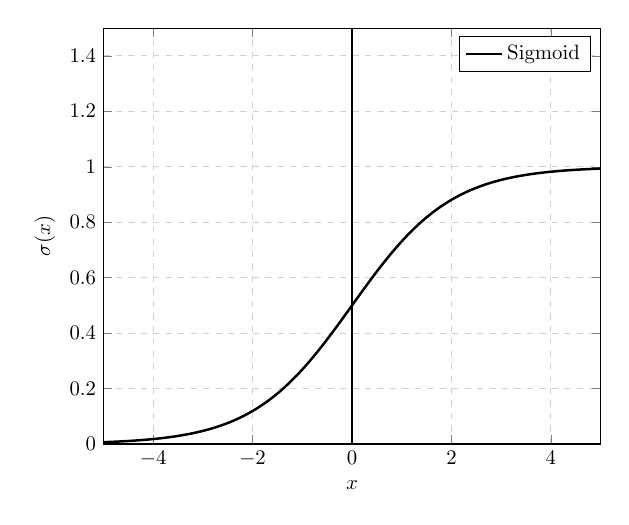
\begin{tikzpicture}[scale=0.75]
			\begin{axis}[
				xlabel=$x$, ylabel=$\sigma(x)$,
				xmin=-5, xmax=5,
				ymin=0, ymax=1.5,
				grid=major, grid style={dashed, gray!35},
			]
			\addplot[black, samples=500, very thick] {1/(1+exp(-x))};
			
			% This plots a horizontal line from xmin to xmax
			\draw[semithick] (axis cs:\pgfkeysvalueof{/pgfplots/xmin}, 0) -- (axis cs:\pgfkeysvalueof{/pgfplots/xmax}, 0);
			
			% This plots a vertical line from ymin to ymax
			\draw[semithick] (axis cs:0, \pgfkeysvalueof{/pgfplots/ymin}) -- (axis cs:0, \pgfkeysvalueof{/pgfplots/ymax});
			
			\addlegendentry{Sigmoid}
			\end{axis}
		\end{tikzpicture}
		
		\caption{Sigmoid activation function.}
		\label{fig:sigmoid}
	\end{figure}

	\subsubsection{Tanh}
	
	Tanh is similar to the sigmoid but has an output range of [-1, 1] which in turn means, the output values are zero-centered. Thus, strongly negative inputs to the tanh will map to negative outputs and zero-valued inputs will map to near-zero outputs. Hence, it can overcome the vanishing gradient problem.
	
	\begin{equation}
		f(x) = \tanh(x) = \frac{\sinh(x)}{\cosh(x)} = \frac{e^{x} - e^{-x}}{e^{x} + e^{-x}}
	\end{equation}

	\input{tanh.tex}
	
	\subsubsection{ReLU}
	
	One of the most popular and widely used activation function is the rectified linear unit (ReLU). This function whilst simple, it is proven to be very effective with fast convergence and it is mainly used as an activation function for the hidden layers.
	
	\begin{equation}
		f(x) = \max(0, x) =
		\begin{cases}
			0, & \text{if x $<$ 0} \\
			x, & \text{if x $\geq$ 0}
		\end{cases}
	\end{equation}
	
	\begin{figure}[H]
		\centering
		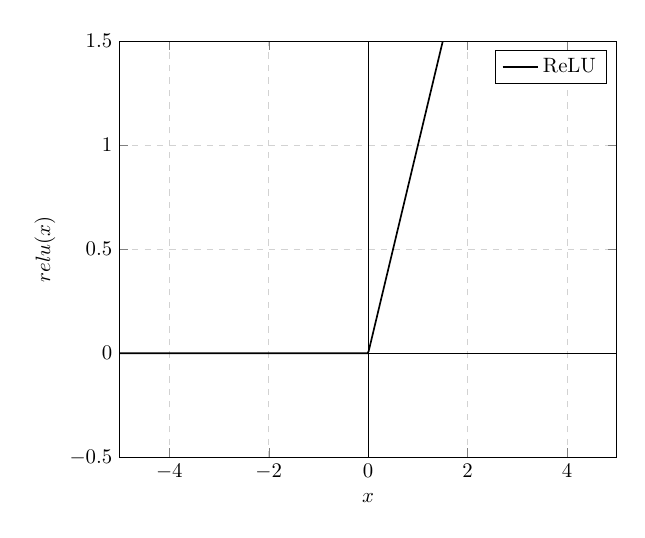
\begin{tikzpicture}[scale=0.75]
		\begin{axis}[
			xlabel=$x$, ylabel=$relu(x)$,
			xmin=-5, xmax=5,
			ymin=-0.5, ymax=1.5,
			grid=major, grid style={dashed, gray!35},
		]
		\addplot[black, samples=500,  thick] {x * (x > 0)};
		
		% This plots a horizontal line from xmin to xmax
		\draw[semithick] (axis cs:\pgfkeysvalueof{/pgfplots/xmin}, 0) -- (axis cs:\pgfkeysvalueof{/pgfplots/xmax}, 0);
		
		% This plots a vertical line from ymin to ymax
		\draw[semithick] (axis cs:0, \pgfkeysvalueof{/pgfplots/ymin}) -- (axis cs:0, \pgfkeysvalueof{/pgfplots/ymax});
		
		\addlegendentry{ReLU}
		\end{axis}
		\end{tikzpicture}
		
		\caption{Rectifier Linear Unit activation function - ReLU.}
		\label{fig:relu}
	\end{figure}
	
	\subsection{Network Training}
	
	Training a neural network simply means to adjust the weights of the connections between \textit{neurons}. At the beginning, the weights of the connections are initialized randomly. This obviously means that the neural network is going to produce bad results. Thus, in order for the neural network to be used adequately for the required task, it needs to be trained to find the proper weights.\par
	
	\subsubsection{Backpropagation}
	
	The most popular algorithm used for the training of a neural network is \textit{Backpropagation}. This algorithm requires a measure of the network's output error which is given by the \textit{loss function} denoted as $\mathcal{L}$. Its ultimate goal is to minimize this loss function $\mathcal{L}$ in weight space, by using a \textit{gradient} based optimizer such as \textit{Stochastic Gradient Descend (SGD)}, \textit{Adam}, \textit{RMSProp} or others \cite{gradient_descent}.
	The general idea of gradient descent based minimizers, is to iteratively take steps proportional to the negative of the gradient of the target function $\mathcal{L}$.
	
	\vspace*{0.5cm}
	
	\noindent Backpropagation algorithm can be summarized in this three steps:
	
	\begin{enumerate}
		\item \textbf{Forward Pass:} The input is given to the network via the input layer. These inputs are propagated through the network and their activations are computed and stored at each layer.
		
		\item \textbf{Error Calculation:} After the forward pass, the network uses the loss function $\mathcal{L}$ to compute the error by comparing the prediction with the target value (supervised learning), as a means to estimate its performance. If \textit{MSE} is used as the loss function then $\mathcal{L}$ is given by the following equation:
		
		\begin{equation}
			\mathcal{L} = \frac{1}{N}\sum_{i=1}^{N}(output_{i} - target_{i})^{2}
		\end{equation}
		
		\noindent where $N$ denotes the number of neurons in the output layer.
		
		\item \textbf{Backward Pass:} At this step the partial derivative of the loss function $\mathcal{L}$ with respect to the network weights is computed and then an update procedure is initiated which adjusts the weights of the neurons in each layer in a backward manner. Each weight is updated using the following equation:
		
		\begin{equation}
			W_{new} = W_{old} - \gamma \frac{\partial \mathcal{L}}{\partial W_{old}}
		\end{equation}
		
		\noindent where $\gamma$ represents the learning rate, i.e., a hyper-parameter that controls the magnitude of the weight updates.
		Finally, it should be noted that in order to effectively compute the partial derivatives for the backward pass, the chain rule is used:
		
		\begin{equation}
			\frac{\partial x}{\partial z} = \frac{\partial x}{\partial y} \cdot \frac{\partial y}{\partial z}
		\end{equation}
		
	\end{enumerate}
	
	\newpage
	
	\subsubsection{Supervised Learning}
	
	In this type of learning, the network receives both the inputs and the output targets usually called the (\textit{ground truth}) of each training set. Thus for each input, the output of the network, can be compared with the expected result and the network's weights can be adjusted accordingly.
	
	\subsubsection{Unsupervised Learning}
	
	The goal of unsupervised learning is to infer useful information or patterns from a dataset without any guidance. It is called unsupervised because unlike supervised learning, the network is not given any labeled data, which means that there is no correct answer to compare the prediction.
	
	\subsection{Regularization}
	
	Regularization is a technique used in deep learning in order to prevent the model from \textit{over-fitting}. \textit{Over-fitting} occurs when the neural network tries to model the \textit{training-data} too closely in an extent, that impacts negatively its ability and performance for predictions on new data. Out of all the available methods in the literature we list only the ones that are used on this thesis.
	
	\subsubsection{Dropout}
	
	Dropout \cite{dropout} is a technique where a random fraction of neurons are \textit{"dropped"} or \textit{"cut-off" } during the training phase. In essence, this means that at each training step, randomly selected \textit{neurons} are kept with probability $p$ or removed from the network along with their incoming and outgoing connections, with probability $q=1-p$.
	
	\begin{figure}[H]
		\centering
		\includegraphics[scale=0.35, keepaspectratio]{dropout.jpg}
		\caption[Neural network model with Dropout]{Neural network model with Dropout, in the right image crossed neurons are dropped. (Source: \cite{eff_backprop}).}
		\label{fig:dropout}
	\end{figure}

	\subsubsection{Early Stopping}
	
	Early stopping is another technique used in deep learning to prevent the model from overfitting. Essentially, in this technique we need to keep a portion of our training dataset as a validation set. Then we need to constantly monitor the validation set error and whenever this error improves, we store a copy of the models parameters. Hence, when the training algorithm stops we return to the saved parameters rather than the latest ones. The stopping criteria for the training algorithm is when the model stops improving on the validation set i.e. validation error increases, for a specified number of epochs or iterations, usually called the \textit{"patience"}.
	
	\begin{figure}[H]
		\centering
		\includegraphics[scale=0.7, keepaspectratio]{early_stopping.jpg}
		\caption[Early stopping]{Early stopping technique to stop training exactly when validation set error starts to increase.}

		\label{fig:early_stop}
	\end{figure}
	
	\subsection{Neural Network Architectures}
	
	As mentioned earlier artificial neural networks are organized in layers composed of \textit{neurons}. Depending on the problem at hand, connections can be made from neurons of one layer to another or/and between \textit{neurons} at the same layer. This provides a flexibility to the neural network, allowing it to better adapt at a specific task.
		
	\subsubsection{Feedforward Neural Networks (FNN)}
	
	The Feedforward neural network (FNN) depicted in Figure (\ref{fig:fnn}) below, is the simplest type of artificial neural networks. In this type of networks information strictly flows in one direction, from the input-layer to the output-layer. There aren't any feedback loops in the network, which in turn means that the output of every layer doesn't affect the same layer.
	
	\begin{figure}[H]
			\centering
			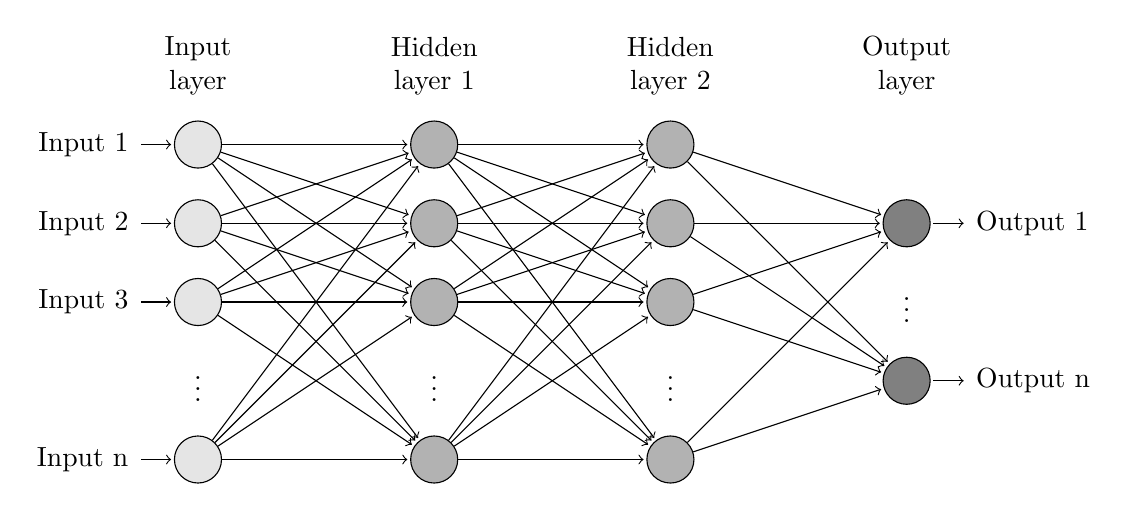
\begin{tikzpicture}[shorten >=1pt,->, node distance=\layersep]
			\tikzstyle{every pin edge}=[<-, shorten <=1pt]
			\tikzstyle{neuron}=[circle, draw=black, minimum size=17pt, inner sep=0pt]
			\tikzstyle{input neuron}=[neuron, fill=black!10];
			\tikzstyle{hidden neuron}=[neuron, fill=black!30];
			\tikzstyle{output neuron}=[neuron, fill=black!50];
			\tikzstyle{annot} = [text width=4em, text centered]
			
			% Draw the input nodes, name contains the string 1,2,...,n and \x contains the offset in number 0,1,2,3,4
			\foreach \name [count=\x from 0] in {1,...,4,n} {
				\ifnum \x=3
					\node at (0, -\x) {$\vdots$};
				\else
					\node[input neuron, pin=left:Input \name] (I-\name) at (0, -\x) {};
				\fi
			}
			
			% Draw the hidden nodes
			\foreach \name [count=\x from 0] in {1,...,4,n} {
				\ifnum \x=3
					\node at (\layersep, -\x) {$\vdots$};
				\else
					\node[hidden neuron] (H1-\name) at (\layersep, -\x) {};
				\fi
			}
		
			% Draw the hidden nodes
			\foreach \name [count=\x from 0] in {1,...,4,n} {
				\ifnum \x=3
					\node at (2*\layersep, -\x) {$\vdots$};
				\else
					\node[hidden neuron] (H2-\name) at (2*\layersep, -\x) {};
				\fi
			}
			
			% Draw the output layer nodes
%			\node[output neuron, pin={[pin edge={->}]right:Output}, right of=H2-2] (O) {};
			\foreach \name [count=\x from 1] in {1,2,n} {
				\ifnum \x=2
					\node at (3*\layersep, -\x) {$\vdots$};
				\else
					\node[output neuron,  pin={[pin edge={->}]right:Output \name}] (O-\name) at (3*\layersep, -\x) {};
				\fi
			}
			
			% Connect every node in the input layer with every node in the
			% 1 hidden layer.
			\foreach \source [count=\xs from 0] in {1,...,4,n} {
				\foreach \dest [count=\xd from 0] in {1,...,4,n} {
					\ifnum \xd=3
					% do nothing
					\else
						\ifnum \xs=3
						% do nothing
						\else
							\path (I-\source) edge (H1-\dest);
						\fi
					\fi
				}
			}
		
			% Connect every node in the input layer with every node in the
			% 2 hidden layer.
			\foreach \source [count=\xs from 0] in {1,...,4,n} {
				\foreach \dest [count=\xd from 0] in {1,...,4,n} {
					\ifnum \xd=3
						% do nothing
						\else
							\ifnum \xs=3
							% do nothing
							\else
								\path (H1-\source) edge (H2-\dest);
							\fi
					\fi
				}
			}

			% Connect every node in the 2 hidden layer with the output layer
			\foreach \source [count=\xs from 0] in {1,...,4,n} {
				\foreach \dest [count=\xd from 1] in {1,2,n} {
					\ifnum \xd=2
						% do nothing
					\else
						\ifnum \xs=3
							% do nothing
						\else
							\path (H2-\source) edge (O-\dest);
						\fi
					\fi
				}
			}
			
			% Annotate the layers
			\node[annot, above of=H1-1, node distance=1cm] (hl1) {Hidden layer 1};
			\node[annot, above of=H2-1, node distance=1cm] (hl2) {Hidden layer 2};
			\node[annot, left of=hl1] {Input layer};
			\node[annot, right of=hl2] {Output layer};
			\end{tikzpicture}
		
			\caption{Feedforward neural network.}
			\label{fig:fnn}
		\end{figure}
	
	\subsubsection{Recurrent Neural Networks (RNN)}
	
	Conventional neural networks make the assumption that every input element is independent from each other. This means that after processing one element there isn't any kind of information maintained, thus making them unsuitable for sequential data like time series.\par
	
	A \textit{recurrent neural network} (RNN) is a network that can overcome this limitation. More specifically, this network has \textit{feedback loops} in it, making it capable of preserving historical information from previous timesteps.
	
	\begin{figure}[H]
		\centering
		\includegraphics[scale=0.5, keepaspectratio]{rnn.png}
		\caption[Standard recurrent neural network]{A recurrent neural network and its unfolded version to show how the network's \textit{memory} is built (Source: \cite{nature_dl}).}
		\label{fig:rnn}
	\end{figure}
	
	In general the RNN, takes as input a sequence of vectors $x_t = \left \{ x_1, x_2, ..., x_T \right \}$ computes the hidden states $s_t = \left \{ s_1, s_2, ..., s_T\right \}$ and finally outputs $o_t = \left \{ o_1, o_2, ..., o_T\right\}$ for every time step $t$, $t \in \left \{1, 2, ..., T\right\}$. The hidden states represent the \textit{memory} of the network and are computed by passing the weighted input at the current timestep $x_t$ with the weighted hidden state of the previous timestep $s_{t-1}$ through an activation function $f$.\par
	
	\vspace*{0.5cm}
	
	\noindent This procedure can be described mathematically as:
	
	\begin{equation}
		s_{t} = f(Ux_{t} + Ws_{t-1} + b_s)
	\end{equation}
	
	\begin{equation}
		o_{t} = f(Vs_{t} + b_o)
	\end{equation}
	
	\vspace*{0.5cm}
	\noindent where $U, W, V$ are the weight matrices which are the same for each timestep, $b_{*}$ are the biases and $f$ is a non-linear activation function.\par
	
	A recurrent neural network can be unfolded as depicted in Figure (\ref{fig:rnn}) and can be treated as a standard feedforward network that can be trained in a way similar to backpropagation. This approach is called Backpropagation Through Time (BPTT) \cite{BPTT}. Furthermore, even though RNNs can model sequence data decently they are not capable of maintaining long-term dependencies \cite{rnn_learn_difficulties}.

	\subsubsection{Long-Short Term Memory Networks (LSTM)}
	
	In order to overcome the aforementioned problem in the training phase of the RNN, Hochreiter and Schmidhuber introduced the LSTM architecture \cite{LSTM}. This architecture later got many updates and refinements from many researchers. One of the most notable additions to the vanilla architecture of the LSTM, was that of Schmidhuber, Gers and Cummins which included the \textit{forget} gate \cite{LSTM_forget}.\par
	The LSTM architecture is very similar to that of the RNN but with the exception that each neuron is replaced by an LSTM unit \textemdash Figure (\ref{fig:lstm_unit}), which is a composite unit composed of a \textit{memory cell} and three \textit{gates}: input, output and forget gates.
	
	\begin{enumerate}
		
		\item \textbf{Forget Gate:} The forget gate applies a sigmoid function on the weighted sum of the  input in the current timestep $x_{t}$ and the output of the previous step $h_{t-1}$ and outputs a value between [0, 1]. This effectively decides, which information is going to be removed from the cell state. A value of 0 indicates that the information should be completely removed and a value of 1 exactly the opposite.
		
		\begin{equation}
			f_{t} = \sigma(W_{f}x_{t} + R_{f}h_{t-1} + b_{f})
		\end{equation}
		
		\item \textbf{Input Gate:} The input gate applies a sigmoid function on the weighted sum of the  input in the current timestep $x_{t}$ and the output of the previous step $h_{t-1}$, to ascertain which values to be updated on the cell state $C_{t}$.
		This information is combined with the new candidate values for the cell state, denoted as $\widetilde{C_{t}}$, by passing $x_{t}$ and $h_{t-1}$ through a tanh function.
		
		\begin{equation}
			i_{t} = \sigma(W_{i}x_{t} + R_{i}h_{t-1} + b_{i})
		\end{equation}
		
		\begin{equation}
			\widetilde{C_{t}} = tanh(W_{c}x_{t} + R_{c}h_{t-1} + b_{c})
		\end{equation}
		
		\item \textbf{Memory Cell:} The memory cell is updated by forgetting the information that is no longer required from the previous time step and the information that is relevant in the current timestep.
		
		\begin{equation}
			C_{t} = f_{t} \odot C_{t-1} + i_{t} \odot \widetilde{C_{t}}
		\end{equation}
		
		\item \textbf{Output Gate:} The output gate applies a sigmoid function on the weighted sum of $x_{t}$ and $h_{t-1}$ in order to control what information should flow out of the LSTM unit. The result of this gate is then passed through a tanh function to produce the output of the LSTM unit $h_t$, at the current timestep $t$.
		
		\begin{equation}
		o_{t} = \sigma(W_{o}x_{t} + R_{o}h_{t-1} + b_{o})
		\end{equation}
		
		\begin{equation}
		h_{t} = tanh(C_{t}) \odot o_{t}
		\end{equation}
	\end{enumerate}
	
	\newpage
	
	It should be noted that in the equations above, $\odot$ is element-wise multiplication (Hadamard product) and $W_{*}, R_{*}$ and $b_{*}$ represent the input weights, the recurrent weights and the biases respectively.\\
	
	\vspace*{0.5cm}
	
	% Makebox required because image bigger than \textwdith and couldn't be centered appropriately
	\begin{figure}[H]
		\makebox[\textwidth][c]{
			\includegraphics[scale=0.7, keepaspectratio]{LSTM_unit.png}
		}
		\caption[Internal structure of an LSTM unit]{Internal structure of an LSTM unit (Source: Colah's blog \cite{colah_blog}).}
		\label{fig:lstm_unit}
	\end{figure}

	\subsubsection{Gated Recurrent Unit (GRU)}
	
	The Gated Recurrent Unit was introduced by Kyunghyun Cho \cite{GRU} and is another variant of RNNs that follows closely the architecture of the LSTM. Both variants, can track long-term dependencies while mitigating the problems of the training phase in RNNs \cite{rnn_learn_difficulties}.\par
	
	Similarly to the LSTM unit, the GRU unit employs gating mechanisms to modulate the flow of information inside the unit. It combines the input and forget gates into a single \textit{update gate} and has an additional \textit{reset gate}. Additionally, the GRU does not maintain a \textit{cell state} and exposes its full content without any adjustment. That being said, the GRU unit is simpler than the LSTM and has fewer parameters which makes it more computational efficient.\par
	
	\begin{enumerate}
		\item \textbf{Update Gate:} The update gate $z_t$ decides how much the unit updates its content or information from the previous step. It applies a sigmoid function to the weighted sum of the input at the current timestep $x_t$ and the previous output $h_{t-1}$.
		
		\begin{equation}
			z_t = \sigma(W_{z}x_{t} + R_{z}h_{t-1})
		\end{equation}
		
		\item \textbf{Reset Gate:} The reset gate $r_t$ decides how to combine the new input with the previous memory. Similarly to the update gate, it applies a sigmoid function to the weighted sum of the input at the current timestep $x_t$ and the previous output $h_{t-1}$.
		
		\begin{equation}
			r_t = \sigma(W_{r}x_{t} + R_{r}h_{t-1})
		\end{equation}
		
		\item \textbf{Output:} The output of the GRU unit $h_t$ at time $t$ is a linear interpolation between the previous output $h_{t-1}$ and the candidate output $\tilde{h_{t}}$.
		
		\begin{equation}
			\tilde{h_{t}} = \tanh(W_{h}x_{t} + R_{h}(r_{t} \odot h_{t-1}))
		\end{equation}
		
		\begin{equation}
			h_{t} = (1 - z_{t}) \odot h_{t-1} + z_{t} \odot \tilde{h_{t}}
		\end{equation}
	\end{enumerate}

	It should be noted that in the equations above, $\odot$ is element-wise multiplication (Hadamard product) and $W_{*}, R_{*}$ represent the input weights and the recurrent weights respectively.
		
	\begin{figure}[H]
		\centering
		\includegraphics[width=0.6\textwidth, height=0.6\textheight, keepaspectratio]{GRU_unit.png}
		\label{fig:GRU}
		\caption[Internal structure of a GRU unit]{Internal structure of a GRU unit (Source: Colah's blog \cite{colah_blog}).}
	\end{figure}
	
	\newpage
%	
	\section{Data Preprocessing Techniques} \label{data_preprocessing}
	
	In deep learning, the raw input data have to undergo some transformations prior to inserting them to the network. This procedure has proven to significantly improve the convergence as well as the performance of the model \cite{eff_backprop}.
	
	\subsection{Normalization}
	
	Normalization also known as "Min-Max Scaling" is the process of rescaling the data from the original scale into the desired scale, which is usually [0, 1] or [-1, 1]. Of course, a linear scaling like this requires that the minimum and maximum values can be found. \par
	
	\vspace*{0.5cm}
	
	\noindent The equation to normalize the data in the range [a, b] is the following:
	
	\begin{equation} \label{eq:normalization}
	%		x_{t}' = (b - a) \frac{x_t - x_{min}}{x_{max} - x_{min}} + a
		X_t' = (b - a) \frac{X_t - X_{min}}{X_{max} - X_{min}} + a
	\end{equation}
	
	\vspace*{0.5cm}
	
	\noindent A variant of this method, called "Mean Normalization" subtracts the mean value $\mu$, instead of the minimum. Thus, Equation (\ref{eq:normalization}) becomes:
	
	\begin{equation}
		X_t' = (b - a) \frac{X_t - \mu}{X_{max} - X_{min}} + a
	\end{equation}
	
	%	In our experiments we decided to normalize the input data into the range of [-1, 1] which is equivalent to the range of the activation function "tanh", used in the LSTM networks. This is proven to be more efficient for the convergence of the network \cite{eff_backprop}.
	
	\subsection{Standardization}
	
	The goal of standardization is to rescale the input features, so that they have the properties of a standard normal distribution, i.e. zero mean and unit standard deviation, $\mu=0 $ and $ \sigma=1$. Of course, this method requires that the mean and standard deviation of the observable values can be found.\par
	
	\vspace*{0.5cm}
	
	\noindent The equation to standardize the data is the following:
	
	\begin{equation} \label{eq:standardization}
	%		x_{t}' = \frac{x_t - \mu}{\sigma}
		X_t' = \frac{X_t - \mu}{\sigma}
	\end{equation}
	
	\vspace*{0.5cm}
	
	\noindent where $\mu$ is the mean and $\sigma$ is the standard deviation of the data.
	
	% \noindent is required in order to be vertical aligned
	\noindent\begin{minipage}{0.5\linewidth}
		\centering
		\begin{equation}
			\mu = \frac{1}{N} \sum_{t=1}^{N}X_t
		\end{equation}
	\end{minipage}
	\begin{minipage}{0.5\linewidth}
		\centering
		\begin{equation}
			\sigma = \sqrt {\frac{1}{N} \sum_{t=1}^{N}(X_t - \mu)^{2}}
		\end{equation}
	\end{minipage}
	
%	\subsection{Differencing}
%	
%	The majority of the forecasting methods/algorithms require the data to be stationary (section \ref{stationarity}). In practice though, it usually happens that the time series exhibits a \textit{trend} or/and \textit{seasonality} which makes it hard for the model to learn and achieve good performance.\par
%	
%	One technique to make the time series stationary is differencing. Differencing computes the differences between consecutive observations to replace the actual values.
%	A differenced series $D_t$ is created from the original $X_t$ according to:
%	
%	\begin{equation}
%	D_t = X_t - X_{t-1}, \  t \in \left\{ 1, ..., T \right\}
%	\end{equation}
%	
%	By differencing the time series it helps to stabilize the mean and make it stationary. Furthermore, differencing can be applied multiple times if there is still evidence of non-stationarity.\par
%	
%	Finally, unlike traditional methods like ARIMA, RNNs and especially LSTM networks are very capable of learning non-linearities and long-term dependencies. Thus, stationarity is not required for the time series prediction with LSTM networks, but it can improve the performance of the model. \todo{Check if this paragraph needed here or in methodology}
	
	\newpage
	
	\section{Software Tools}
	
	\subsection{Deep Learning Frameworks} \label{seciton:dl_frameworks}
	A deep learning framework is an interface or library that allows developers to easily design, build and evaluate deep learning models, by using a collection of pre-built optimized components. There is a huge collection of deep learning frameworks one can use to develop neural networks, with the most popular listed below.
	
	\subsubsection*{Tensorflow}
	
	\href{https://www.tensorflow.org/}{\textbf{Tensorflow}} is an open source library  for high performance numerical computation using data flow graphs. Its flexible architecture allows easy deployment of computations across various platforms such as CPUs and GPUs. It was developed by Google Brain Team and is one of the most commonly used frameworks today.

	\subsubsection*{Theano}
	
	\href{http://deeplearning.net/software/theano/}{\textbf{Theano}} is a python library that allows you to define, optimize and evaluate mathematical expressions involving multi-dimensional arrays efficiently on either CPU or GPU architectures.
	It was developed by a research group at the University of Montreal and it was one of the first widely used deep learning frameworks.
	
	\subsubsection*{Microsoft Cognitive Toolkit}
	
	\href{https://www.microsoft.com/en-us/cognitive-toolkit/}{\textbf{Microsoft Cognitive Toolkit (CNTK)}} is an open-source software toolkit for commercial-grade distributed deep learning, developed by Microsoft. It describes neural networks as a series of computational steps via a directed graph. It also allows for easy integration with Azure Cloud Services.
	
	\subsubsection*{Keras}
	
	\href{https://keras.io/}{\textbf{Keras}} is a high level deep-learning library in Python that offers a very human-friendly and easily operated interface in order to build neural networks. It's capable of running on top of of either Tensorflow, Theano or Microsoft Cognitive Toolkit. Keras was developed and maintained by Fran\c{c}ois Chollet and has a huge community and support.
	
	\subsection{Scientific Libraries}
	
	Python has a wide variety of libraries that transform it from a general purpose programming language into a very powerful tool for data analysis and visualization. Some of the core libraries used in this thesis and that make this feasible are listed below.
	
	\subsubsection*{NumPy}
	
	\href{http://www.numpy.org/}{\textbf{NumPy}} is the foundational library for scientific computing in Python, and many of the most popular libraries use NumPy arrays as their basic inputs and outputs. In short, NumPy introduces objects for multidimensional arrays and matrices, as well as routines that allow developers to perform advanced mathematical and statistical functions on those arrays.
	
	\subsubsection*{SciPy}
	
	 \href{https://www.scipy.org/}{\textbf{SciPy}} is a collection of mathematical algorithms and high-level functions built on top of NumPy. This package provides efficient numerical routines such as numerical integration, optimization, linear algebra and many others via its submodules.
	
	\subsubsection*{Scikit-learn}
	
	\href{http://scikit-learn.org/stable/}{\textbf{Scikit-learn}} is a python machine learning library that builds on NumPy and SciPy by adding algorithms for common machine learning and data mining tasks such as clustering, regression and classification.
	
	\subsubsection*{Pandas}
	
	\href{https://pandas.pydata.org/}{\textbf{Pandas}} is a software library written for the Python programming language for data manipulation and analysis. In particular, it offers high-level data structures and operations for manipulating numerical tables and time series. 
	
	\subsubsection*{Matplotlib}
	\href{https://matplotlib.org/}{\textbf{Matplotlib}} is the standard Python library that is used to generate visualizations such as 2D plots and graphs.
	
	\newpage
	
	\section{Methodology}
	
	In this thesis, we decided to use Keras to build the deep learning models for the time series prediction task. In the subsequent sections we briefly explain all the required steps of our implementation.
	
	\subsection{Data Preparation}
	
	\subsubsection{Data Split}
	
	In order to build the model and estimate its performance, we need to split the dataset into three subsets namely the \textit{training, validation} and \textit{test} set.
	
	\begin{itemize}
		\item \textbf{Training Dataset:}
		This set is used solely during the training procedure of the neural network in order to fit the parameters of the model (e.g. weights).
		
		\item \textbf{Validation Dataset:}
		This set is mainly used to provide an unbiased evaluation of the model fit on the training dataset. This set is used to tune the \textit{hyperparameters} of the neural network (e.g. number of hidden units).
		
		\item \textbf{Test Dataset:}
		This set is comprised by previously unseen data and it is used to assess the predictive performance of the final model.
	\end{itemize}

	\vspace*{0.5cm}
	
	This method is called Holdout Validation and the general procedure one follows when doing this split on the dataset is depicted in Figure (\ref{fig:train_valid_test}) below.
	
	\begin{figure}[H]
		\centering
		\includegraphics[width=0.75\textwidth, height=0.75\textheight, keepaspectratio]{train_valid_test.png}
		\caption{Holdout validation.}
		\label{fig:train_valid_test}
	\end{figure}
	
	\subsubsection{Supervised Learning} \label{subsection:supervised}
	
	In order to train the neural network, the time series data needs to be reformed and framed as a supervised learning task. A common approach is to use a \textit{sliding window} over the dataset in order to create input-output pairs. For instance, if we have the series $X = \left\{X_1, X_2, ..., X_{10}\right\} $ and we would like to use the last three observations (timesteps) in order to predict the next value in the series, then we need to produce the following sequences:

	\begin{table}[H]
		\centering
		\begin{tabular}{@{} cc @{}}
			\toprule
			Input & Output \\
			\midrule
			$\left[X_1, X_2, X_3 \right]$ & $X_4$ \\
			
			$\left[X_2, X_3, X_4 \right]$ & $X_5$ \\
			
			$\left[X_3, X_4, X_5 \right]$ & $X_6$ \\
			
			$\left[X_4, X_5, X_6 \right]$ & $X_7$ \\
			
			$\left[X_5, X_6, X_7 \right]$ & $X_8$ \\
			
			$\left[X_6, X_7, X_8 \right]$ & $X_9$ \\
			
			$\left[X_7, X_8, X_9 \right]$ & $X_{10}$ \\	
			\bottomrule
		\end{tabular}
		\caption{Time series conversion to supervised learning.}
		\label{table:supervised}
	\end{table}

	\subsubsection{Data Preprocessing - Transformation}

	Before we input the raw data in the network they have to undergo some transformations as mentioned in Section (\ref{data_preprocessing}). For the LSTM network, all the input time series have been normalized in the range [-1, 1] to match the output range of the activation function $\tanh$. This is accomplished by using Equation (\ref{eq:normalization}).\par
	
	It should be noted that in order to evaluate the model predictions and gather metrics, the predictions need to be inverted back to the original scale. This is accomplished by using a reverse operation of Equation (\ref{eq:normalization}). \par
	
	It is also really important to not leak any information when doing this operation from the test dataset during training. Thus, in order to normalize or standardize the time series, one should estimate the parameters of the equations only from the training dataset.
	
	\newpage
	
	\subsection{Keras Implementation Details}
	
	Working with LSTM in Keras is not that straightforward and requires some attention when building the model. In the following sections, we briefly discuss these tricky parts.
	
%	\paragraph{{\small LSTM Input/Output}}
	\subsubsection{LSTM Input/Output}

	To start with, the LSTM layer requires the input data to be in the form of a three dimensional array with dimensions [batch\_size, timesteps, features].
	\begin{enumerate}
		\item { \textbf{Batch\_size}}: is the number of samples in a forward/backward pass before a weight update.
		
		\item { \textbf{Timesteps}}: is the number of past observations to use (i.e. lookback or lags).
		
		\item {\textbf{Features}}: is the number of features for every timestep (1 for univariate or n if multivariate).
	\end{enumerate}
	
	The output of the LSTM layer by default is a 2D array with dimensions [batch\_size, units] or [batch\_size, timesteps, units] in case the argument \textit{"return\_sequences"} in the LSTM layer, is set to True. This option is mainly used when multiple LSTM layers are stacked together, in order for the next LSTM layer to obtain the whole sequence (timesteps) from the previous.
	
%	\paragraph{{\small LSTM State}}
	\subsubsection{LSTM State}
	
	Another option in the LSTM layer is the parameter \textit{"stateful"}. Even though, LSTM layers are inherently stateful, this option allows batches of samples to share the values of their hidden states. Thus, if this option is enabled the hidden state of $i_{th}$ sample in the previous batch $k$ will be provided as initial state to the $i_{th}$ sample in the subsequent batch $k+1$.\par
	
	It should be noted though, that in case a network is stateful the batch\_size has to be a divisor of the size of all the datasets (train, validation, test). Thus, an additional pre-processing step has to be made for the time series data that might require to truncate the last batches of the datasets.\par
	
	Additionally, after the network is rendered stateful, there should be special care on when the model should reset the the states. It is common to reset the states after the whole sequence has been processed. Thus, for time series forecasting, we should reset the states after each epoch (i.e. a complete forward/backward pass of all the samples).
	
	\newpage
	
%	\paragraph{Callbacks}
	\subsubsection{Callbacks}
	
	Keras allows the creation of callbacks in order to make changes to the network during training.
	In thesis, the following callbacks are created/used:
	
	\begin{enumerate}
		\item \textbf{EarlyStopping}: To monitor the validation loss and stop training when there is no improvement for a number of epochs.
		
		\item  \textbf{ModelCheckpoint}: This callback saves the weights as well as all the information regarding the training state of the model in a special file (HDF5 format).
		
		\item \textbf{ReduceLROnPlateau}: This is used to reduce the learning rate of the optimizer in case there is no improvement in the validation loss for a number of epochs.
		
		\item \textbf{ResetStateCallback}: This callback is mainly created to reset the states of the model at the end of each epoch (in case the model is stateful).
		
		\item \textbf{CVSLogger}: Callback in order to store the evaluation metrics for each epoch, during training.
		
	\end{enumerate}

	\subsection{Hyperparameter Tuning}
	The whole complexity of the experiments with ANNs is the process of tuning the hyperparameters (e.g. number of neurons, number of layers, learning rate, epochs etc.). In our experiments we manually tuned the hyperparameters of the model via trial and error.
	For deeper and more complex networks, one can look into more time-consuming and exhaustive searching methods like grid-search, random-search or bayesian optimization \cite{Koch2017AutomatedHT, hyperparameter_tuning_blog}.
	
	\newpage
	
	\section{Experiments and Results}
	
	As mentioned earlier, our deep learning models are built with Keras. Keras allows the use of different backends (frameworks) such as Tensorflow, Theano and CNTK to handle all the low-level operations.
	In this section, we test the performance of the aforementioned frameworks in terms of training speed and prediction accuracy for out-of-sample forecasts (i.e. forecasts on the testing dataset). We will focus on univariate time series \textemdash Table (\ref{table:datasets}) and a method for one-step ahead forecasts will be employed.\par
	
	\vspace*{0.5cm}
	
	  \textemdash \textit{It should be noted, that all frameworks are CPU only variants and have been installed from the official sites (see Section \ref{seciton:dl_frameworks}) following the proposed guidelines and using the default configurations.}
	
	\subsection{Setup}
	
	The following tables contain the detailed specifications of the machine and the frameworks that are used in the experiments.

	\vspace*{0.5cm}

	\begin{table}[H]
		\centering
		\small
		% This removes the padding on vertical edges the @{} @{}
			\begin{tabular}{@{} L{4cm} L{4cm}  @{}}
				\toprule
				\multicolumn{2}{c}{System Details} \\
				\midrule
				Platform                   & Linux x86\_64 \\
				Distribution              & Ubuntu 16.04.5 LTS \\
				CPU Model                & Intel i7-4700MQ \\
				Number of Cores      & 4 \\
				Number of Threads  & 8 \\
				CPU Frequency         & 2.40 - 3.40 GHz \\
				Memory (RAM)          & 8 GB \\
				\bottomrule
			\end{tabular}
		\caption{Machine specifications.}
		\label{table:machine_specs}
	\end{table}

	\begin{table}[H]
			\centering
			\small
			\begin{tabular}{@{} L{4cm} L{4cm} @{}}
				\toprule
				Framework & Version \\
				\midrule
				Keras            & 2.2.2 \\
				Tensorflow   & 1.9.0 \\
				Theano         & 1.0.2 \\
				CNTK			& 2.5.1 \\
				\bottomrule
			\end{tabular}
			\caption{Deep learning frameworks version.}
			\label{table:frameworks_versions}
	\end{table}

	\newpage
	
	\subsection{Datasets}
	
	The datasets used in the experiments are publicly available and their details are listed in Table (\ref{table:datasets}) below.
	
	\begin{table}[H]
		\centering
		\begin{tabular}{@{} L{3cm} L{5cm} L{1cm} c L{2cm} @{}}
			\toprule
			Dataset Name & Abstract & Size & Attributes & Source \\
			\midrule
			Beijing PM2.5 Dataset & This hourly data set contains the PM2.5 data of US Embassy in Beijing. Meanwhile, meteorological data from Beijing Capital International Airport are also included. & 43824 & 13 &  \href{https://archive.ics.uci.edu/ml/datasets}{UCI Machine Learning Repository} \\
			Internet traffic data (in bits) from an ISP & This dataset contains aggregated traffic in the United Kingdom academic network backbone. It was collected between 19 November 2004, at 09:30 hours and 27 January 2005, at 11:11 hours. Data is collected at five minute intervals. & 19888 & 1 & \href{https://datamarket.com/data/set/232g/internet-traffic-data-in-bits-from-an-isp-aggregated-traffic-in-the-united-kingdom-academic-network-backbone-it-was-collected-between-19-november-2004-at-0930-hours-and-27-january-2005-at-1111-hours-data-collected-at-five-minute-intervals#!ds=232g&display=line}{Time Series Data Library} \\
			Zürich monthly sunspot numbers & This dataset describes a monthly count of the number of observed sunspots for over 230 years (1749-1983). & 2820 & 1 &
			\href{https://datamarket.com/data/set/22ti/zuerich-monthly-sunspot-numbers-1749-1983#!ds=22ti&display=line}{Time Series Data Library}
			\\
			\bottomrule			
		\end{tabular}
	\caption{Datasets details.}
	\label{table:datasets}
	\end{table}

	The Beijing PM2.5 dataset contains also meteorological data, but we're interested in forecasting the PM2.5 concentration, thus we are going to drop all the other attributes. Furthermore, we can observe that the dataset contains some missing values hence, an additional pre-processing step has to be done to remove these rows. The Zürich and Internet traffic datasets, are left as is because there are no missing values.\par
	
	\newpage
	
	\subsubsection{Dataset Visualizations}
	
	In order to get a visual grasp of the patterns that govern the time series, the datasets are plotted over their whole range \textemdash Figures (\ref{fig:beijing_plot} - \ref{fig:zurich_plot}).
	
	\begin{figure}[H]
		\centering
		\includegraphics[width=\textwidth, height=\textheight, keepaspectratio]{datasets/beijing.pdf}
		\caption{Beijing PM2.5 dataset visualization.}
		\label{fig:beijing_plot}
	\end{figure}
	
	\begin{figure}[H]
		\centering
		\includegraphics[width=\textwidth, height=\textheight, keepaspectratio]{datasets/internet.pdf}
		\caption{Internet traffic dataset visualization.}
		\label{fig:internet_plot}
	\end{figure}

	\begin{figure}[H]
		\centering
		\includegraphics[width=\textwidth, height=\textheight, keepaspectratio]{datasets/zurich.pdf}
		\caption{Zürich sunspots dataset visualization.}
		\label{fig:zurich_plot}
	\end{figure}

	\newpage

	\subsection{Model Details}
	
	The same model is used for all the datasets, in order to compare the scalability of the frameworks in terms of the length of the datasets. Additionally, after experimentation with the tuning procedure of the hyperparameters, we chose the ones that lead the model to produce the best prediction performance on all validation datasets.\par
	
	The predictor is a stateful multi-layered model that consists of two stacked LSTM layers with 128 and 256 neurons respectively and a Dense layer (fully connected layer) with a single neuron to produce a single prediction (one-step ahead forecasting). The first LSTM layer returns as an output the whole sequence (timesteps), while the second one returns only the last step, thus dropping the temporal dimension. In-between layers we added a dropout layer of 0.2, in order to prevent the model from overfitting. The model is trained for 30 number of epochs with early-stopping and a batch size of 128. The objective loss function is MSE and RMSprop \cite{rmsprop} is used as the network's optimizer with a learning-rate of 0.001. Furthermore, the learning rate is monitored and is reduced by a factor of 0.5 in case there is no improvement in the validation loss for 5 epochs. The time series have been converted to input-output pairs (supervised learning) with a number of $24$ past timesteps and one output, with a process like the one depicted in Section (\ref{subsection:supervised}) \textemdash Table (\ref{table:supervised}). We use 70\% of data for training, 10\% for validation and the last 20\% to test the prediction performance. The model's architecture as well as its input/output dimensions are depicted in Figures (\ref{fig:lstm_keras_io} - \ref{fig:lstm_keras_architecture}) below.
	
	\begin{figure}[H]
		\centering
		\includegraphics[height=0.6\textheight, width=0.6\textwidth, keepaspectratio]{LSTM_keras.png}
		\caption{Model's architecture with each layer's  I/O dimensions.}
		\label{fig:lstm_keras_io}
	\end{figure}
	
	\begin{figure}[H]
	\centering
	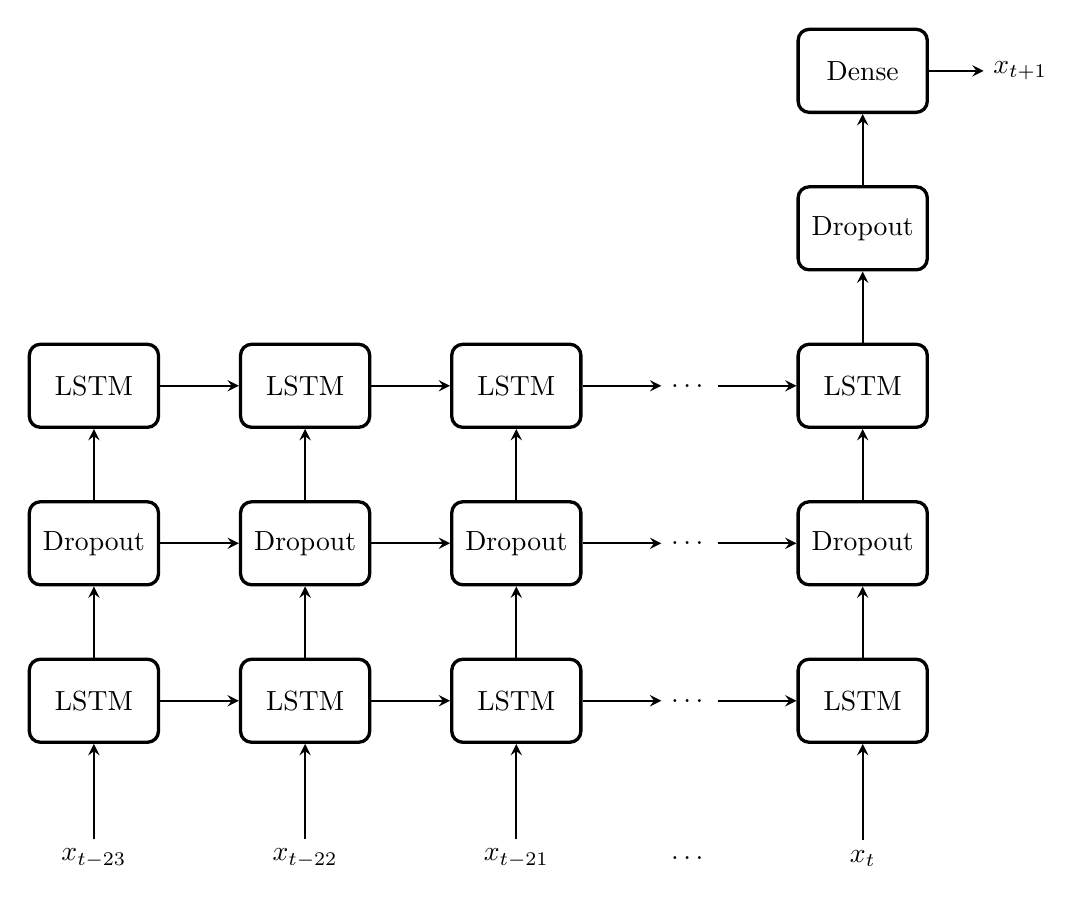
\begin{tikzpicture}[>=stealth',
		punktchain/.style={
			rectangle, 
			rounded corners, 
%			 fill=black!10,
			draw=black, very thick,
			text width=4em, 
			minimum height=3em, 
			text centered},
		arrow/.style={thick, draw, -stealth},
		every join/.style={thick, -stealth},
		start chain=1 going right, start chain=2 going right,
		start chain=3 going right,
		node distance=2cm and 1cm]
		\node[punktchain, on chain=1, join] (a) {LSTM};
		\node[punktchain, on chain=1, join] (b) {LSTM};
		\node[punktchain, on chain=1, join] (c) {LSTM};
		\node[on chain, on chain=1, join] (d) {$\dots$};
		\node[punktchain, on chain=1, join] (e) {LSTM};
		\node[below of=a] (xt23) {$x_{t-23}$};
		\node[below of=b] (xt22) {$x_{t-22}$};
		\node[below of=c] (xt21) {$x_{t-21}$};
		\node[below of=d] (xt20) {$\dots$};
		\node[below of=e] (xt) {$x_{t}$};
		\draw [arrow] (xt23) -- (a);
		\draw [arrow] (xt22) -- (b);
		\draw [arrow] (xt21) -- (c);
		\draw [arrow] (xt) -- (e);
		\node[punktchain, on chain=2, above of=a, join] (da) {Dropout};
		\node[punktchain, on chain=2,  join] (db) {Dropout};	
		\node[punktchain, on chain=2,  join] (dc) {Dropout};
		\node[on chain=2,join] (dd) {$\dots$};
		\node[punktchain, on chain=2,  join] (de) {Dropout};
		\draw [arrow] (a) -- (da);
		\draw [arrow] (b) -- (db);
		\draw [arrow] (c) -- (dc);
		\draw [arrow] (e) -- (de);
		\node[punktchain, on chain=3, above of=da, join] (la) {LSTM};
		\node[punktchain, on chain=3, join] (lb) {LSTM};
		\node[punktchain, on chain=3, join] (lc) {LSTM};
		\node[on chain, on chain=3, join] (ld) {$\dots$};
		\node[punktchain, on chain=3, join] (le) {LSTM};
		\draw [arrow] (da) -- (la);
		\draw [arrow] (db) -- (lb);
		\draw [arrow] (dc) -- (lc);
		\draw [arrow] (de) -- (le);
		\node[punktchain, above of=le] (dfinal) {Dropout};
		\draw [arrow] (le) -- (dfinal);
		\node[punktchain, above of=dfinal] (dense) {Dense};
		\draw [arrow] (dfinal) -- (dense);
		\node [right of=dense] (output) {$x_{t+1}$};
		\draw [arrow] (dense) -- (output);
		\end{tikzpicture}
		
		\caption[An illustration of the LSTM model]{An illustration of the LSTM model. It takes as input the past 24 observations (timesteps) and produces an output sequence to the next layers. Finally, the output of the last cell of the second LSTM layer is used as input to the fully connected layer to produce a scalar output prediction. In-between layers we've introduced a Dropout layer in order to prevent the model from overfitting.}
		\label{fig:lstm_keras_architecture}
\end{figure}

%	In the previous subsection we stated that the final layer is a fully connected layer with a single neuron which produces a single output. In order to make predictions for many steps ahead in a one shot manner, we use the previous model with some minor modifications. These modifications, include the option \textit{return\_sequences=True} in the last LSTM layer which in turn means that the last \textit{Dense} layer (fully connected layer) will output not a single prediction but \textit{timesteps} predictions (many-to-many). Alternatively, we could use the previous model as is and employ an \textit{Iterative approach} for multi-step ahead predictions.
		
	\newpage
	
	\subsection{Evaluation Metrics and Results}
	
	To assess the performance of the frameworks for the LSTM model, we will use three different metrics, namely the Mean Absolute Error (MAE) Equation (\ref{eq:MAE}), the Root Mean Square Error (RMSE) Equation (\ref{eq:RMSE}) and the time it took for the model to train on the training dataset for 30 epochs.
	
	\vspace*{0.5cm}
	
	\begin{table}[H]
		\centering
		\footnotesize
		\begin{tabular}{@{} L{1.8cm} L{1cm} L{1cm} L{1cm} L{1cm} L{1cm} L{1cm} L{1cm} L{1cm} L{1cm} @{}}
			\toprule
			Dataset & \multicolumn{3}{c}{Beijing PM2.5} &  \multicolumn{3}{c}{Internet Traffic} & \multicolumn{3}{c}{Zürich Sunspots} \\
			\cmidrule(lr){2-4}
			\cmidrule(lr){5-7}
			\cmidrule(lr){8-10}
			Metrics & MAE & RMSE & Time & MAE & RMSE & Time & MAE & RMSE & Time \\
			\midrule
			Tensorflow & 12.30 & 21.75 & 16m59s & 62.15 & 84.56 & 7m29s & 14.06  & 19.00 & 1m0s \\
			Theano & 11.88 & 21.59 & 27m14s & 60.17 & 81.86 & 14m57s & 14.16 & 19.23 & 2m7s \\
			CNTK & 12.19 & 21.85 &  33m48s & 61.97 & 84.60 & 16m38s & 13.43  & 18.28 & 2m14s \\
			\bottomrule
		\end{tabular}
		\caption{Framework evaluation metrics of the LSTM for every dataset}
		\label{table:lstm_metrics}
	\end{table}

	\vspace*{0.5cm}
	
	Additionally, we trained with TensorFlow a GRU network as an exact replica of the LSTM, to compare their performance. From Table (\ref{table:lstm_gru_metrics}), it is clear that GRU achieves better score for the given datasets while being faster during training, indicating that it might be better candidate for modeling the time series.
	
	\vspace*{0.5cm}

	\begin{table}[H]
		\centering
		\footnotesize
		\begin{tabular}{@{} L{1.8cm} L{1cm} L{1cm} L{1cm} L{1cm} L{1cm} L{1cm} L{1cm} L{1cm} L{1cm} @{}}
			\toprule
			Dataset & \multicolumn{3}{c}{Beijing PM2.5} &  \multicolumn{3}{c}{Internet Traffic} & \multicolumn{3}{c}{Zürich Sunspots} \\
			\cmidrule(lr){2-4}
			\cmidrule(lr){5-7}
			\cmidrule(lr){8-10}
			Metrics & MAE & RMSE & Time & MAE & RMSE & Time & MAE & RMSE & Time \\
			\midrule
			LSTM   & 12.30 & 21.75 & 16m59s & 62.15 & 84.56 & 7m29s & 14.06 & 19.00 & 1m0s \\
			GRU     & 11.94 & 21.69 & 13m35s & 57.91 & 78.76 & 6m31s & 13.41 & 18.39 & 0m55s \\
			\bottomrule
		\end{tabular}
		\caption{Tensorflow: LSTM vs GRU evaluation metrics for every dataset}
		\label{table:lstm_gru_metrics}
\end{table}
	
	\newpage
	
	\subsection{Predictions Visualization}
	
	In the following subsections we will illustrate the first 300 out-of-sample predictions of the GRU model for every dataset. The GRU model was chosen because it achieved the best MAE and RMSE scores, as depicted in Table (\ref{table:lstm_gru_metrics}).
	
	\subsubsection{Beijing PM2.5 Dataset}
	
	Figure (\ref{fig:beijing_test_preds}) depicts the first 300 continuous plots of one-step-ahead forecasted values and the actual values on the test dataset.
	
	\begin{figure}[H]
		\centering
		\includegraphics[width=\textwidth, height=\textheight, keepaspectratio]{plots/beijing/beijing_300_test_preds.pdf}
		\caption[Out-of-sample one-step-ahead forecasts on the Beijing PM2.5 dataset]{One-step-ahead predictions on the Beijing PM2.5 test dataset. Predictions are represented with red color and actual values with blue.}
		\label{fig:beijing_test_preds}
	\end{figure}
	
	\newpage
	
	\subsubsection{Internet Traffic Dataset}
	
	Figure (\ref{fig:internet_test_preds}) depicts the first 300 continuous plots of one-step-ahead forecasted values and the actual values on the test dataset.
	
	\begin{figure}[H]
		\centering
		\includegraphics[width=\textwidth, height=\textheight, keepaspectratio]{plots/internet/internet_300_test_preds.pdf}
		\caption[Out-of-sample one-step-ahead forecasts on the Internet Traffic dataset]{One-step-ahead predictions on the  Internet traffic test dataset. Predictions are represented with red color and actual values with blue.}
		\label{fig:internet_test_preds}
	\end{figure}

	\newpage

	\subsubsection{Zürich Sunspots Dataset}

	Figure (\ref{fig:zurich_test_preds}) depicts the first 300 continuous plots of one-step-ahead forecasted values and the actual values on the test dataset.
	
	\begin{figure}[H]
		\centering
		\includegraphics[width=\textwidth, height=\textheight, keepaspectratio]{plots/zurich/zurich_300_test_preds.pdf}
		\caption[Out-of-sample one-step-ahead forecasts on the Zürich sunspots dataset]{One-step-ahead predictions on the Zürich sunspots test dataset. Predictions are represented with red color and actual values with blue.}
		\label{fig:zurich_test_preds}
	\end{figure}

	\newpage

	\section{Conclusion}
	
	In this thesis we presented the relevant theory, of time series and deep learning, that is required in order to build a model to perform time series forecasting.
	Subsequently, we presented the state-of-the-art deep learning architectures for sequence based tasks (LSTM, GRU), their inner workings as well as methods that are widely used in deep learning.
	Additionally, we showed the steps of how to manipulate time series and frame them in a form that is suitable for the LSTM model's training.
	Furthermore, many of the implementation details of Keras are presented, which are required in order to build the LSTM, to feed the time series data to the LSTM as well as to monitor its training.
	Finally, these models were trained with the available deep learning frameworks that serve as the backend engine of Keras and comparisons were made in terms of prediction accuracy and training speed for different datasets and for different network architectures (LSTM - GRU).\par
	
	For the last part, even though different frameworks use slightly different implementations of the mathematical operations, the results gathered from the experiments are approximately the same, except for the training speed. This is mainly due to the different optimizations of the mathematical libraries used in the background that handle the matrix and linear algebra operations. Additionally, from the experiments presented in Table (\ref{table:lstm_metrics}) we can clearly see that CNTK is the slowest in terms of training speed, with Theano being a little bit faster than the former and TensorFlow being the fastest.\par
	
	As of the comparison of the LSTM versus the GRU network, it seems that GRU is less computationally expensive than LSTM, mainly because of the fewer parameters which result in a faster training speed. It is also evident that the GRU can achieve better predictions than the LSTM, having better evaluation scores as indicated by the results presented in Table (\ref{table:lstm_gru_metrics}).\par
	
	To sum up, it seems that the winner of the frameworks comparison is Google's TensorFlow, as it achieved approximately the same evaluation score, but it was approximately 2x faster than the others. Hence, to build LSTM and GRU models for time series prediction, TensorFlow seems to be the most suitable framework as the backend engine of Keras in a CPU (non-GPU) setup, by using the default configurations provided in the installation guidelines of each framework.
	
	\newpage
	
	% Used to include references wihtout citing them inside document
	\nocite{*}
	
	\bibliography{thesis}
	\bibliographystyle{unsrtnat}
	
	% Add References into the TOC
	\addcontentsline{toc}{section}{References}

\end{document}